\documentclass[12pt, twoside]{article}
\usepackage[francais]{babel}
\usepackage[T1]{fontenc}
\usepackage[latin1]{inputenc}
\usepackage[left=1cm, right=1cm, top=1cm, bottom=1cm]{geometry}
\usepackage{float}
\usepackage{graphicx}
\usepackage{array}
\usepackage{multirow}
\usepackage{amsmath,amssymb,mathrsfs}
\usepackage{soul}
\usepackage{textcomp}
\usepackage{eurosym}
 \usepackage{variations}
\usepackage{tabvar}

\begin{document}


\section*{\center{Devoir maison 10}}

\textit{Devoir � rendre sur feuille double grand format pour le
\ul{jeudi 14 mai 2009}. }

\subsection*{Exercice 1}

\begin{tabular}{cc}
\begin{minipage}{5cm}
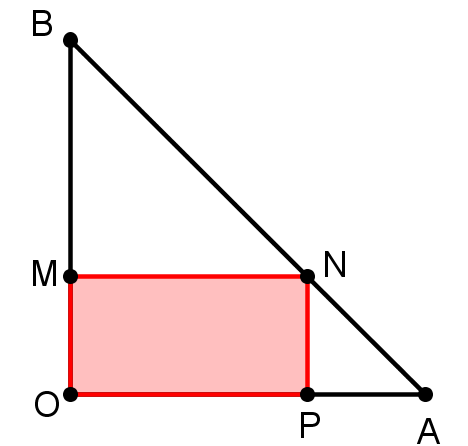
\includegraphics[width=4cm]{images/ex1.png}
\end{minipage}
\begin{minipage}{13cm}
Le triangle $AOB$ est rectangle et isoc�le en $O$ avec $OA=OB=10cm$. $M$ �tant
un point quelconque du segment $[OB]$, la parall�le � $(OA)$ passant par $M$
coupe $[AB]$ au point $N$ et la parall�le � $(OB)$ passant par $N$ coupe $[OA]$
au point $P$. Dans ces conditions, le quadrilat�re $OMNP$ est un rectangle.
Nous allons nous int�resser � l'aire de ce rectangle.


\end{minipage}
\end{tabular}

\bigskip


\begin{enumerate}
  \item Soit $x$ la longueur du segment $[OM]$. Exprimer en fonction de $x$ les
  longueurs $AP$ et $OP$.
  \item On d�signe par $S(x)$ la fonction d�finissant l'aire du rectangle
  $OMNP$. Calculer $S(x)$ en fonction de $x$.
  \item On consid�re la fonction $f$ d�finie sur l'intervalle $[0;10]$ par
  $f(x)=-x^2+10x$.
  \begin{enumerate}
    \item Soit $a$ et $b$ deux nombres de l'intervalle $[0;10]$. Montrer que
    $f(b) -f(a)=(b-a)(10-(a+b))$.
    \item D�montrer que la fonction $f$ est croissante sur l'intervalle
    $[0;5]$. Quel est son sens de variation sur l'intervalle $[5;10]$,
    d�montrer-le.
    \item Donner le tableau de variation de la fonction $f$. En d�duire la
    position du point $M$ correspondant � une aire $S(x)$ maximum. Pr�ciser
    cette aire.
  \end{enumerate}
  \end{enumerate}


\subsection*{Exercice 2}

Un petit balcon rectangulaire a pour aire $2m^2$ et pour p�rim�tre $6m$.
  Quelles sont les dimensions \textbf{exactes} du balcon? (Les r�sultats doivent
  �tre justifi�s.)
  
  
  \medskip
  
  \textit{Indication:} On pourra se ramener � une �tude de fonctions.  


 \subsection*{Exercice 3}
 
 Il s'agit de l'exercice 4 de la photocopie distribu�e.
 
 \medskip
 
 \ul{Remarques}: 
 Expliquer votre strat�gie et justifier toutes les associations trouv�es. Une
 association sans justification donnera 0 point.
 
 La calculatrice peut vous aider � conjecturer ces associations (mais en aucun
 cas � les d�montrer).

\end{document}
